\documentclass[border=5mm]{standalone}
\usepackage{tikz}

\definecolor{cof}{RGB}{219,144,71}
\definecolor{pur}{RGB}{186,146,162}
\definecolor{greeo}{RGB}{91,173,69}
\definecolor{greet}{RGB}{52,111,72}
\definecolor{white}{RGB}{255,255,255}
\definecolor{black}{RGB}{0,0,0}

\begin{document}

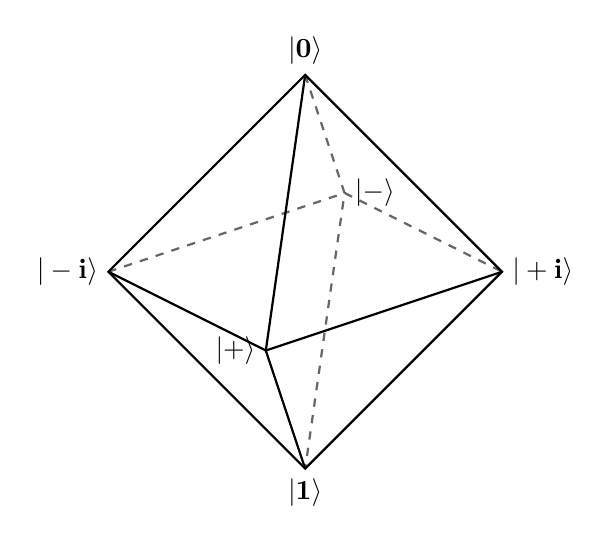
\begin{tikzpicture}[thick,scale=5]
    \coordinate[label=left:$\mathbf{|-i\rangle}$] (A1) at (0,0);
    \coordinate[label=right:$\mathbf{|-\rangle}$] (A2) at (0.6,0.2);
    \coordinate[label=right:$\mathbf{|+i\rangle}$] (A3) at (1,0);
    \coordinate[label=left:$\mathbf{|+\rangle}$] (A4) at (0.4,-0.2);
    \coordinate[label=above:$\mathbf{|0\rangle}$] (B1) at (0.5,0.5);
    \coordinate[label=below:$\mathbf{|1\rangle}$] (B2) at (0.5,-0.5);

    \begin{scope}[thick,dashed,,opacity=0.6]
        \draw (A1) -- (A2) -- (A3);
        \draw (B1) -- (A2) -- (B2);
    \end{scope}
    \draw (B1) -- (A1) -- (B2) -- (A3) --cycle;
    \draw (A1) -- (A4) -- (A3);
    \draw (B1) -- (A4) -- (B2);
\end{tikzpicture}

\end{document}